%%%%%%%%%%%%%%%%%%%%%%%%%%%%%%%%%%%%%%%%%%%%%%%%%%%%%%%%%%%%%%
%% LaTeX template for the science justification to be       %%
%%     submitted as part of a regular ALMA proposal.        %%
%% This template should also be used for a ToO, DDT, or     %%
%%     mm-VLBI ALMA proposal, but NOT for Large Programs    %%
%%     (these have a separate template with more sections)  %%
%%                                                          %%
%%                      ALMA Cycle 9                        %%
%%                                                          %%
%%%%%%%%%%%%%%%%%%%%%%%%%%%%%%%%%%%%%%%%%%%%%%%%%%%%%%%%%%%%%%

%%%%%%%%%%%%%%%%%%%%%%%%%%%%%%%%%%%%%%%%%%%%%%%%%%
%%%%% How to convert this document to PDF %%%%%%%%
%%%%%%%%%%%%%%%%%%%%%%%%%%%%%%%%%%%%%%%%%%%%%%%%%%

% If your figures are stored as PostScript files, you can use the 
% following commands to generate a PDF file of your proposal:

%% latex file.tex
%% dvips file.dvi
%% ps2pdf file.ps file.pdf 


% If your figures are PDF images or bitmap pictures in PNG, JPG, or GIF format,
% you can use the pdflatex command to generate a PDF file from this template
% (note, however, that the pdflatex command does not handle PostScript files):

% pdflatex file.tex

% Warnings: 
%           1. You must make sure that PDF output generated from this
%              template is complete both when displayed with a viewer 
%              (acroread, for example) and when printed on paper.
%              LaTeX installations vary greatly and therefore it might 
%              not be possible to get all proposals to come out 
%              correctly with a single text page layout. 
%              In some cases you will have to adjust the 
%              \topmargin=-7mm command in the template to center the 
%              text vertically in the page.  
%           2. The scientific justification, figures, tables, references,
%              and public outreach statement must all fit within the
%              4-page limit.
%           3. You are free to include colour images in your proposal justification.
%              Proposals are distributed to ALMA Review Panels and to distributed
%              peer review reviewers in electronic form.
%              However, the scientific content of the images should still remain
%              clear when displayed or printed in black and white.
%           4. This template is for regular, ToO, DDT, or mm-VLBI ALMA proposals,
%              but NOT for Large Programs: these have a separate template with
%              more sections, and is available from the ALMA Science Portal


%%%%%%%%%%%%%%%%%%%%%%%%%%%%%%%%%%%%%%%%%%%%%%
%%%%% Default format: 12pt single column %%%%%
%% 12pt is the minimum font size allowed !! %%
%% This applies to everything, including    %%
%% references, figure captions, and tables  %%
%% ==> Proposals not compliant to this will %%
%%     be rejected. See Section 5.3.1 in    %%
%%     the ALMA Proposer's Guide            %%
%%%%%%%%%%%%%%%%%%%%%%%%%%%%%%%%%%%%%%%%%%%%%%

\documentclass[12pt,a4paper]{article}  %% DO NOT CHANGE to 11pt or less !

\usepackage[dvipdfmx]{graphics, graphicx}
% if you on overleaf...
\usepackage{color}
% if you on local...
% \usepackage[dvipdfmx]{color}
\usepackage[version=4]{mhchem}
\usepackage{amsmath,amssymb}
\usepackage{natbib}
\usepackage{aas_macros}
\usepackage{compactbib}
% \usepackage{txfonts}
\usepackage{threeparttable}
\usepackage{xspace}
\usepackage{enumitem}
\usepackage{adjustbox}
\usepackage{wrapfig}
\usepackage[colorlinks=true,citecolor=blue]{hyperref}

%%%%%%%%%%%%%%%%%%%%%%%%%%%%
%%%%%% Page dimensions %%%%%
%%%%%%  DO NOT CHANGE  %%%%%
%%%%%%%%%%%%%%%%%%%%%%%%%%%%

\textheight=247mm
\textwidth=180mm
\topmargin=-7mm
\oddsidemargin=-10mm
\evensidemargin=-10mm
\parindent 10pt

%%%%%%%%%%%%%%%%%%%%%%%%%%%%%
%%%%% Start of document %%%%% 
%%%%%%%%%%%%%%%%%%%%%%%%%%%%%

\begin{document}
\pagestyle{plain}
\pagenumbering{arabic}
 
% The title, abstract and list of investigators should NOT be included in the
% Scientific justification. The title and abstract are put automatically on the cover page.

%%%%%%%%%%%%%%%%%%%%%%%%%%%%%%%%%%%%%%%%%
%%%%% Body of science justification %%%%%
%%%%%%%%%%%%%%%%%%%%%%%%%%%%%%%%%%%%%%%%%

%% ENTER TEXT, FIGURES AND TABLES BELOW
%% Minimum font size for all text, references, figure captions, and tables is 12pt
%% Proposals not compliant to this will be rejected. See Section 5.3.1 in the ALMA Proposer's Guide.

\section{Scientific justification}
\subsection{Background}
Deuterium enrichment (the enhanced abundance of deuterated isotopologues) is a common phenomenon seen in Solar System material. For example, seawater on Earth and water in comets and meteorites have a molecular D/H ratio of $\sim$10$^{-4}$ \citep{Mumma11}, significantly enhanced with respect to the interstellar elemental abundance ($\sim$10$^{-5}$). Because deuterium enrichment is caused by exchange reactions in low temperature environments, it has been inferred that at least some Solar System material could originate from the interstellar medium such as molecular clouds. Deuterium enrichment is expected in the cold outer region of protoplanetary disks as well. %In particular, a key question is whether the chemical composition is inherited from the ISM or significantly modified during the planet formation process \citep[e.g.][]{Oberg21_review}. 
Since protoplanetary disks are the birthplaces of planetary bodies, e.g., planets and comets, it is important to investigate deuterium chemistry in disks to understand the origin and thermal history of molecules that are eventually incorporated into planetary bodies.

Indeed, recent observations have shown a rich deuterium chemistry in protoplanetary disks. The spatial distribution of deuterated molecules such as DCN, DCO$^+$, and N$_2$D$^+$ have been mapped, and their formation pathways have been inferred from their abundances and temperature structures in the disks \citep[e.g.,][]{Huang17, Salinas17, Oberg21_TWHya, Cataldi21}. The deuterium chemistry in protoplanetary disks is, however, still not fully understood due to the limited number of spatially resolved observations for different molecular species. \textbf{We propose to observe the deuterated hydrocarbons C$_2$D and $c$-C$_3$HD with a spatial resolution of 0\farcs3 toward three protoplanetary disks in order to reveal the distribution of deuterated hydrocarbons. This will allow us to explore the deuterium chemistry of hydrocarbons in protoplanetary disks for the first time.}


\subsection{Deuterium enrichment processes}
Deuterium enrichment is caused by the difference in zero-point energies between a deuterated molecule and its normal isotopologue. It starts from exchange reactions such as
\begin{align}
    \ce{H3+ + HD &-> H2D+ + H2} + 230\, \mathrm{K} \label{eq:lowpath}\\
    \ce{CH3+ + HD &-> CH2D+ + H2} + 432\, \mathrm{K} \label{eq:highpath1} \\ 
    \ce{C2H2+ + HD &-> C2HD+ + H2} + 550\, \mathrm{K}. \label{eq:highpath2}
\end{align}
%While accurate values of the exothermicity $\Delta E$ depend on the ortho-to-para (o/p) ratio of reactants and products, the values with typical o/p ratios are given above as a reference \cite[][]{Millar89, Roberts00, Nyman19}. 
In general, the backward reactions become active (and thus deuterium enrichment becomes inefficient) as the gas temperature rises. The decline of the D/H ratio with temperature is more significant for \ce{H2D+/H3+} and the molecules produced by the reaction with \ce{H2D+}, due to the relatively low exothermicity of (\ref{eq:lowpath}). Reactions \eqref{eq:highpath1} and \eqref{eq:highpath2}, on the other hand, can maintain relatively high D/H ratio ($\sim 10^{-2}$) even at several tens of K.

%So, far D-bearing molecules detected in disks are HD, DCO$^+$, N$_2$D$^+$, and DCN. HD is the major deuterium carrier and thus is not enriched.
Among the deuterated molecules detected in protoplanetary disks, observations have shown that \ce{N2D+} is abundant only in the cold outer region, which is consistent with the theoretical expectation that it is formed from \ce{H2D+}, i.e., the \ce{N2D+/N2H+} ratio is determined by reaction (\ref{eq:lowpath}) \cite[e.g.,][]{Salinas17}. \ce{DCN} and \ce{DCO+} distributions are extended to the warm inner region compared with \ce{N2D+}, which suggests a contribution of reaction (\ref{eq:highpath1}) \cite[e.g.,][]{Huang17, Oberg21_TWHya, Cataldi21}. \textbf{The contribution of reaction (\ref{eq:highpath2}), on the other hand, has never been investigated observationally in protoplanetary disks.}

\vspace{-1em}
\subsection{Previous observations of hydrocarbons in disks}
Possible probes of reaction (\ref{eq:highpath2}) are hydrocarbons: \ce{C2H} and $c$-\ce{C3H2}. Indeed, the \ce{C2D} ($N$=4--3) line was detected in a line survey toward MWC~480 \citep{Loomis20}.
%Emission lines of \ce{C2H}, in paticular, are known to be bright in disks. 
The velocity-integrated emission maps of the \ce{C2D} line toward MWC~480 as well as the high spatial resolution (0\farcs15-0\farcs3) observations of \ce{C2H} and $c$-\ce{C3H2} lines toward three disks \citep{Guzman21} are presented in Figures \ref{fig:C2D_mom0} and \ref{fig:C2H_garelly}. The \ce{C2H} and $c$-\ce{C3H2} lines are bright at the dust continuum gap, which indicates active carbon-chain chemistry triggered by enhanced UV radiation. From these data, we estimated a disk-averaged \ce{C2D} column density of $\sim2\times10^{13}$\,cm$^{-2}$, and a \ce{C2H} column density of $\sim$10$^{15}$ cm$^{-2}$ at the position of the \ce{C2H} ring; i.e., \ce{C2D/C2H} $\sim 0.02$. The excitation temperature of \ce{C2H} is found to be $\sim$60\,K at the peak of the \ce{C2H} ring by fitting the $N=3$--2 and $N=1$--0 lines. Such a high \ce{C2D/C2H} ratio with a high temperature strongly suggests a contribution to the deuterium enrichment by reaction (\ref{eq:highpath2}). \textbf{The spatial resolution of the \ce{C2D} data ($\sim$1$''$) is, however, not sufficient to constrain the distribution of \ce{C2D} and the \ce{C2D/C2H} ratio in the disk.}

Figure \ref{fig:C2D_model} presents the distribution of the \ce{C2D} abundance and the radial column density profile in a thermo-chemical model of a Herbig Ae disk based on \citet{Aikawa18}. \ce{C2D} is indeed abundant in the warm disk surface due to the contribution of reaction \eqref{eq:highpath2}. The column density is predicted to be $\sim$10$^{13}$\,cm$^{-2}$ at the radial peak, comparable to that measured in MWC~480. Similar results have been obtained in a model of a T Tauri disk.

\begin{figure}[tbph]
\centering
\begin{minipage}[b]{0.35\hsize}
\centering
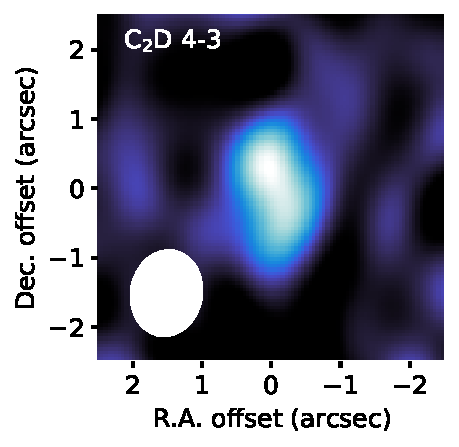
\includegraphics[scale=0.88]{MWC_480_C2D_mom0}
\caption{\em{The velocity-integrated emission map of \ce{C2D} 4--3 toward MWC~480 \citep{Loomis20}. The beam size of 1\farcs2$\times$1\farcs0 is shown in the lower left.}}
%\caption{\em{The zeroth moment maps of \ce{C2H} 3-2, $c$-\ce{C3H2} 7$_{07}$-6$_{06}$, and \ce{C2D} 4-3 toward the MWC~480, HD~163296, and AS~209 disks \cite[][and archival data from project 2018.101055.L]{Loomis20}. The beam is shown in the lower left.}}
\label{fig:C2D_mom0}
\end{minipage}
\hspace{1em}
\begin{minipage}[b]{0.6\hsize}
\centering
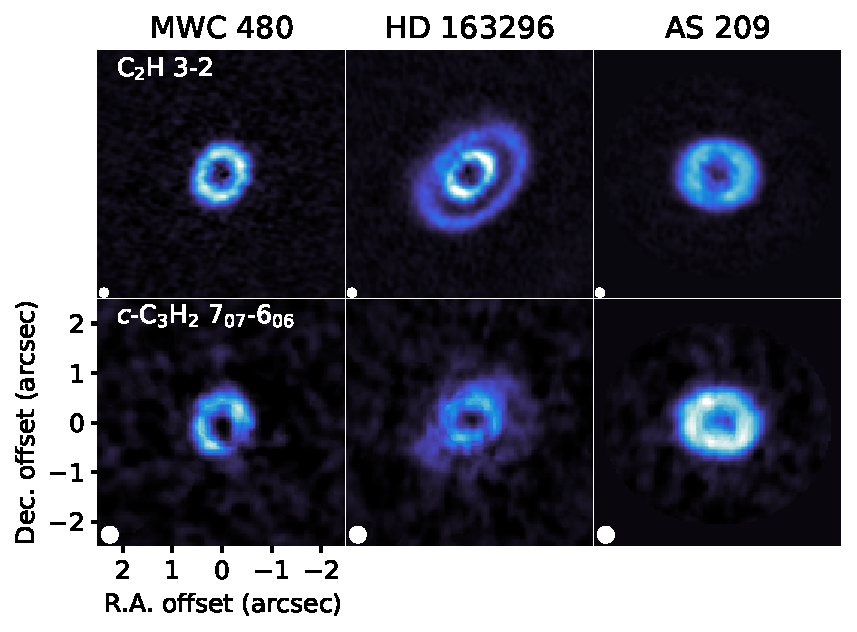
\includegraphics[scale=0.7]{MAPS_hydrocarbon_garelly}
\caption{\em{The velocity-integrated emission maps of \ce{C2H} 3--2 and $c$-\ce{C3H2} 7$_\mathit{0,7}$--6$_\mathit{0,6}$ toward the MWC~480, HD~163296, and AS~209 disks \citep{Guzman21}. The beam sizes of 0\farcs15 (\ce{C2H} 3--2) and 0\farcs3 ($c$-\ce{C3H2} 7$_\mathit{07}$-6$_\mathit{06}$) are shown in the lower left of each panel.}}
\label{fig:C2H_garelly}
\end{minipage}
\end{figure}


\begin{figure}[tbh]
\centering
\begin{minipage}[b]{0.35\hsize}
\centering
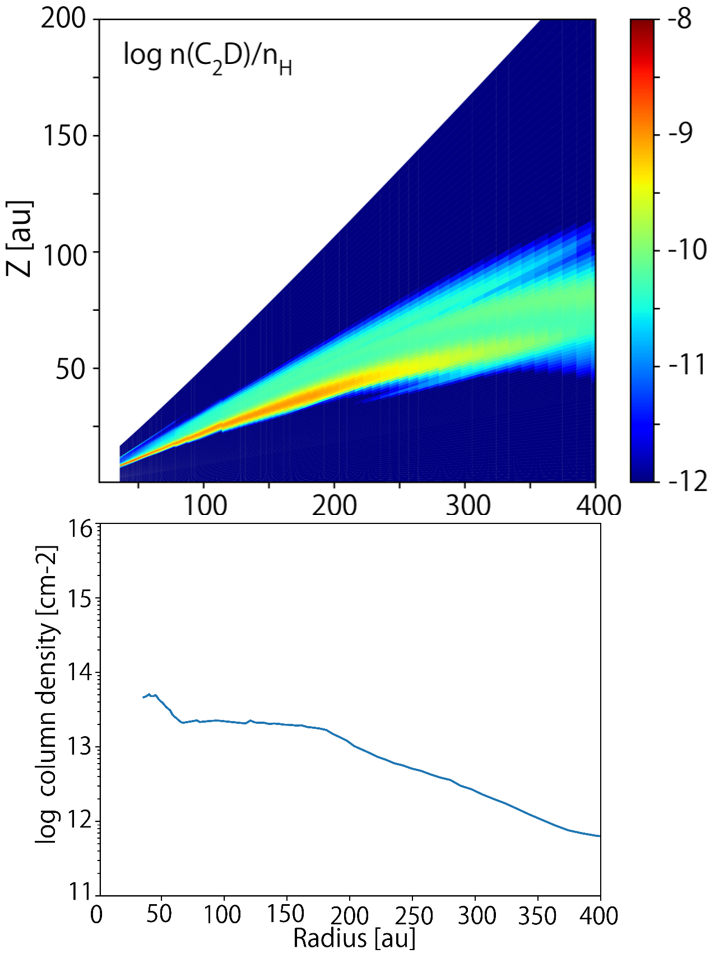
\includegraphics[scale=0.55]{model_C2D_HD163296}
\caption{\em{Model prediction of the spatial distribution of \ce{C2D} (top) and its radial column density distribution (bottom).}}
\label{fig:C2D_model}
\end{minipage}
\hspace{1em}
\begin{minipage}[b]{0.6\hsize}
\centering
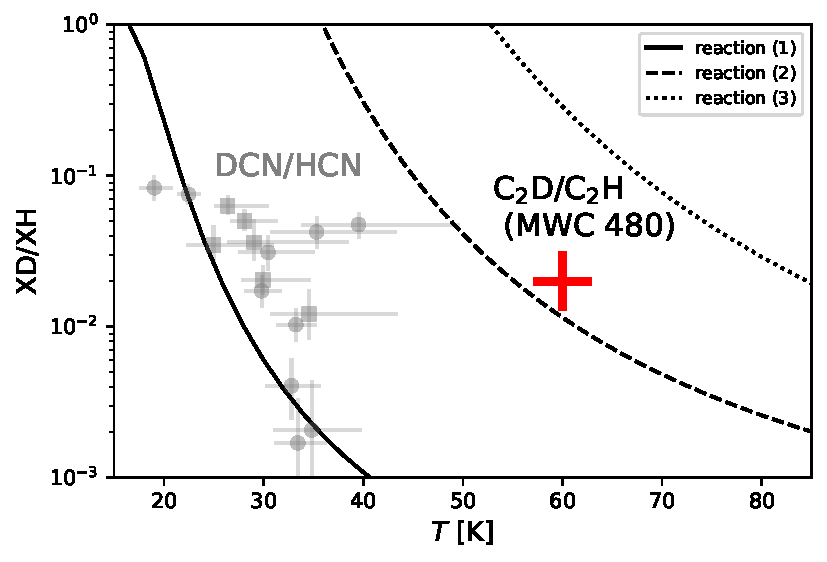
\includegraphics[scale=0.75]{XD2XH_vs_T}
\caption{\em{The molecular D/H ratio as a function of temperature. The three black lines represent the maximum D/H ratio that can be produced by the three reactions shown in equations (\ref{eq:lowpath}), (\ref{eq:highpath1}) and (\ref{eq:highpath2}). We can evaluate the contribution from these reactions by comparing the data points derived from observations with these lines, as demonstrated for HCN and DCN in \citet{Cataldi21}. The red cross presents the data point estimated from the current observation in MWC~480. Since it is above the black dashed line, a contribution from reaction (\ref{eq:highpath2}) is required. %indicating the contribution from reaction \ref{eq:highpath2}
}
}
%\caption{\em{The DCN/HCN column density ratio as a function of temperature (derived from archival data of project 2018.1.101055.L). The black and red lines are upper limits on \ce{DCN/HCN} from reaction \eqref{eq:lowpath} and \eqref{eq:highpath2}, respectively. They show the \ce{H2D+/H3+} and \ce{CH2D+/CH3+} ratios calculated by balancing forward and backward reactions of \eqref{eq:lowpath} and \eqref{eq:highpath1}, respectively. For the latter, estimates by two measured exothermicity (Nyman \& Yu 2019 (solid); Roueff et al. 2013 (dotted)) are shown. Each data point presents the value at a certain radial location derived from line fitting for MWC~480 (brown), HD~163296 (pink), and AS~209 (green). The observed \ce{DCN/HCN} ratio cannot be explained by only reaction \eqref{eq:lowpath}, i.e., a certain contribution from reaction \eqref{eq:highpath1} is needed.}}
\label{fig:DCN_path}
\end{minipage}
\end{figure}



% ALMA uses two systems to review the proposals submitted in the Main Call.
% All proposals requesting less than 50 h on the 12-m Array and all ACA stand-alone proposals requesting less
% than 150 h on the 7-m Array will be reviewed by Distributed peer review (see Section 1.2.1 of the Proposer's Guide).
% All Large Programs will be reviewed by Panels. 
% Additionally, both systems will follow a dual-anonymous procedure, in which the proposers do not know
% who are the reviewers and the reviews do not who are the proposers.
%
% Please refer to the guidelines before writing your proposal:
%     https://almascience.org/proposing/alma-proposal-review/dual-anonymous
%
% In the following part, describe the scientific background of the project,
% pertinent references and previous work relevant to this 
% proposal, together with any figures and tables that you judge necessary
% (use the following two examples as templates, or remove)
% Please do not disclose the name(s) of the proposer(s), and write the proposal in a way
% such that the proposer(s) cannot be identified. 
 
%-----------------------------Figure Start---------------------------

% The 'scale' parameter below allows you to scale the figure so that it fits within the page.
% In this case the figure was scaled to 20% of its original size.
% Note: for .png files one has to use pdflatex, not classic latex
%
% Minimum font size for references: 12pt 
% Proposals not compliant to this will be rejected. See Section 5.3.1 in the ALMA Proposer's Guide.

% \begin{figure}[tbh]
% \includegraphics[scale=0.2]{HL_tau.jpg}
% \caption{\em{ALMA image of the protoplanetary disc surrounding the young star HL Tauri.}}
% \end{figure}
%-----------------------------Figure End------------------------------

%-----------------------------Table Start-----------------------------

% Minimum font size for references: 12pt 
% Proposals not compliant to this will be rejected. See Section 5.3.1 in the ALMA Proposer's Guide.

% \begin{table}[tbh]
% \begin{center}
% \caption[]{\em{Here we show the continuum sensitivity required per band.}}
% \begin{tabular}{cc}
% \hline \noalign {\smallskip}
% Frequency (GHz) & Sensitivity (mJy) \\
% \hline \noalign {\smallskip}
% 300 & 0.10 \\
% 850 & 0.50 \\
% \hline \noalign {\smallskip}
% \end{tabular}
% \end{center}
% \end{table}
%-----------------------------Table End ------------------------------

\section{Description of observations}
We propose to observe \ce{C2D} and $c$-\ce{C3HD} lines in Band 7 at 0\farcs3 resolution toward three protoplanetary disks (Table \ref{tab:disk_sample}), in order to investigate the contribution of reaction \eqref{eq:highpath2} to the deuterium enrichment. Our immediate objectives are:

\textbf{1. Resolving radial distributions of molecular D/H ratios.} Combining the data obtained by this observation with the archival data of \ce{C2H} and $c$-\ce{C3H2} (Figure \ref{fig:C2H_garelly}), we will derive the radial distributions of their molecular D/H ratios resolved at 0\farcs3 (30--50\,au depending on the source).

\textbf{2. Determining molecular D/H ratios as a function of temperature.} By fitting multiple spectral lines simultaneously, we will be able to estimate excitation temperatures and molecular D/H ratios at different radial locations. Thus, \textbf{we will be able to determine the molecular D/H ratios as a function of temperature}, and to discuss the contribution of three reactions (1), (2), and (3). In Figure 4, three lines indicate the maximum molecular D/H ratios that can be produced by these three reactions as functions of temperature. We will constrain the contribution of these three reactions by comparing the data points derived from observation with these lines. For example, the large red cross above the dashed line corresponds to a \ce{C2D/C2H} ratio of 0.02 and a \ce{C2H} excitation temperature of 60\,K estimated from the current data of MWC~480. Such a high ratio with a warm temperature cannot be explained by reactions (\ref{eq:lowpath}) and (\ref{eq:highpath1}) only, i.e., a contribution of reaction (\ref{eq:highpath2}) is needed. This method has already been proven feasible for HCN and DCN \citep{Cataldi21}: in Figure \ref{fig:DCN_path}, it can be seen that a contribution of reaction \eqref{eq:highpath1} is needed to explain the observed DCN/HCN ratios.

\textbf{By combining the information obtained from 1. and 2., we will be able to reveal where in the disk the deuterium enrichment via reaction (3) is active.}

\vspace{1em}
\noindent
\textbf{\underline{Disk sample and spatial resolution}}
Our targets are two Herbig Ae disks, MWC~480 and HD~163296 and one T Tauri disk, AS~209 (Table \ref{tab:disk_sample}). These disks show bright \ce{C2H} and $c$-\ce{C3H2} emission in ring structures (Figure \ref{fig:C2H_garelly}). As summarized in Table \ref{tab:disk_sample}, all of these disks show high \ce{C2H} column densities of 10$^{14-15}$\,cm$^{-2}$ in their rings. However, the excitation temperatures are different among the disks. We can make use of this difference to investigate the dependence of the \ce{C2D/C2H} ratio on temperature as described above. Most interestingly, \ce{C2H} in HD~163296 presents two nested rings where the excitation temperature is different for each ring, allowing us to investigate the difference of deuterium enrichment between the two rings. We note that these nested rings ($\sim$0\farcs4 separation) will be distinguished by our requested spatial resolution of 0\farcs3. %These disks have high \ce{C2H} column densities, as estimated from the archival data: $\sim$10$^{15}$\,cm$^{-2}$ at the radial peak. 
%We note that it is reasonable for \ce{C2D} detection to observe sources with a high \ce{C2H} column density because the abundance of \ce{C2H} (and thus of \ce{C2D}) is sensitively dependent on C/O ratio in the disk. 
%As summarized in Table \ref{tab:disk_sample}, the \ce{C2H} emission distribution shows rings, but the excitation temperatures of \ce{C2H} is different among the disks. We can make use of this difference to investigate the dependence of the \ce{C2D/C2H} ratio on temperature (analogous to what is shown in Figure \ref{fig:DCN_path} for DCN). Most interestingly, HD~163296 presents a clear nested ring structure where the excitation temperature is different for each ring, allowing us to investigate the difference of deuterium enrichment between the two rings. We note that this nested ring will be clearly resolved by our requested spatial resolution of 0.3$''$. %This makes these disks promising targets to detect the deuterated hydrocarbons. We cover both Herbig Ae and T Tauri disks to investigate the dependence of the deuteration on the luminosity of the central star. 
\begin{center}
\begin{threeparttable}[tbh]
\label{tab:disk_sample}
\caption[]{\em{Disk sample}}
\begin{tabular}{cccccc}
\hline \noalign {\smallskip}
Source  & $D$ [pc] & $L_\mathrm{bol}$ [$L_\odot$] & \ce{C2H} structure & $N$(\ce{C2H}) at ring [cm$^{-2}$] & $T_\mathrm{ex}$ at ring [K]\\
\hline \noalign {\smallskip}
MWC~480   & 161.8 & 21  & narrow ring & 10$^{15}$ & 60 \\
HD~163296 & 101.5 & 17  & nested rings & 10$^{15}$, $3\times10^{14}$ \tnote{$\dagger$} & 60, 40 \tnote{$\dagger$} \\
AS~209    & 121   & 1.4 & broad ring & 10$^{15}$ & 40 \\
\hline \noalign {\smallskip}
\end{tabular}
\begin{tablenotes}
\item[$\dagger$] Values at the inner ring and the outer ring, respectively.
\end{tablenotes}
\end{threeparttable}
\end{center}

\noindent
\textbf{\underline{Spectral line selection}}
We chose the \ce{C2D} $N=4$--3 line at 288.5 GHz, which has been detected in MWC~480 by \citet{Loomis20}, as a main target. In order to trace the warm disk surface region where reaction (3) dominates and to achieve a spatial resolution of 0\farcs3 that can resolve the ring structures, we aim to detect the 4--3 line ($E_\mathrm{up} = 35$\,K) rather than the 3--2 line ($E_\mathrm{up} = 20$\,K). Although this line has not been detected in HD~163296 and AS~209, we expect a detection if the \ce{C2D/C2H} ratio is similar to that in MWC~480, considering the similar peak column densities of \ce{C2H} ($\sim$10$^{15}$\,cm$^{-2}$). Even in the case of a non-detection, we can derive upper limits on the \ce{C2D/C2H} ratio, which will allow us to discuss the contribution from three reactions and the variation of deuterium enrichment among the disks.

As a secondary target (not used to estimate the requested sensitivities), we will observe the $c$-\ce{C3HD} line at 286.9 GHz in the same setup. Although $c$-\ce{C3HD} has not been detected in protoplanetary disks, we expect that it will be detected if we assume a $c$-\ce{C3HD}/$c$-\ce{C3H2} ratio similar to starless cores and protostellar phase sources ($\sim$0.1), as measured by \citet{Chantzos18}, since the $c$-\ce{C3H2} column densities measured in the targeted disks are 10$^{12-13}$\,cm$^{-2}$. In the case of non-detection, we can derive upper limits on the $c$-\ce{C3HD}/$c$-\ce{C3H2} ratio, enabling us to discuss the contribution of three deuteration reactions and compare with the early phase deuteration \citep{Chantzos18}. 

\smallskip
\noindent
\textbf{\underline{Analysis techniques}}
We will use several techniques developed recently. We will use the shifting and stacking method \cite[e.g.,][]{Yen16}, which corrects for the Keplerian rotation of the disk, to boost the signal-to-noise ratio of the line profile. Combining our data with the archival data of \ce{C2H} and $c$-\ce{C3H2}, we will fit the stacked spectra of the lines simultaneously to estimate the column densities and excitation temperatures. \citet{Loomis18} presented a matched filter technique for interferometric data to detect weak lines by using data of a bright line with a similar emission distribution as the targeted line, or a simple Keplerian model, as a filter. We will apply this technique to each spectral line. Even if the line is too weak to be analyzed in the image plane (e.g., for $c$-\ce{C3HD}), we can obtain basic information about the spatial distribution by using filters corresponding to different sized disks. 

% Please describe the observations to be made and their specific
% purpose, with a clear explanation of the need for, and 
% appropriateness of, ALMA Cycle 9 data.  


\vspace{-1em}
\section*{References}
\bibliographystyle{aas_compactbib}
\bibliography{reference}

% \section{References}

% List references here
% Minimum font size for references: 12pt 
% Proposals not compliant to this will be rejected. See Section 5.3.1 in the ALMA Proposer's Guide.

% \noindent [1] Author1 et al. year, journal, vol, page

% \noindent [2] Author2 et al. year, journal, vol, page


%%%%%%%%%%%%%%%%%%%%%%%%%%%
%%%%% End of document %%%%%
%%%%%%%%%%%%%%%%%%%%%%%%%%%

\end{document}

